\documentclass[12pt,a4paper]{article}

% =========================================================
% PACKAGES
% =========================================================
\usepackage[utf8]{inputenc}
\usepackage[T5]{fontenc}
\usepackage[vietnamese]{babel}

\usepackage{geometry}
\geometry{margin=2.35cm}

\usepackage{amsmath, amssymb}
\usepackage{graphicx}
\usepackage{booktabs}
\usepackage{array}
\usepackage{float}
\usepackage{enumitem}
\usepackage{xcolor}
\usepackage{hyperref}
\usepackage{fancyhdr}
\usepackage[most]{tcolorbox}
\usepackage{tikz}
\usetikzlibrary{arrows.meta, positioning, shapes.geometric}

% =========================================================
% COLORS
% =========================================================
\definecolor{mainblue}{HTML}{1F4E79}
\definecolor{lightblue}{HTML}{EAF2F8}
\definecolor{mainteal}{HTML}{117A65}
\definecolor{lightteal}{HTML}{E8F6F3}
\definecolor{mainorange}{HTML}{B9770E}
\definecolor{lightorange}{HTML}{FEF5E7}
\definecolor{maingray}{HTML}{34495E}
\definecolor{lightgray}{HTML}{F4F6F7}
\definecolor{mainred}{HTML}{A93226}
\definecolor{lightred}{HTML}{FDEDEC}

% =========================================================
% HYPERREF
% =========================================================
\hypersetup{
    colorlinks=true,
    linkcolor=mainblue,
    citecolor=mainblue,
    urlcolor=mainblue
}

% =========================================================
% HEADER / FOOTER
% =========================================================
\pagestyle{fancy}
\fancyhf{}
\lhead{\textcolor{mainblue}{Báo cáo cập nhật tiến độ}}
\rhead{\textcolor{maingray}{\thepage}}
\setlength{\headheight}{15pt}
\renewcommand{\headrulewidth}{0.4pt}

% =========================================================
% SECTION STYLE
% =========================================================
\usepackage{titlesec}

\titleformat{\section}
  {\Large\bfseries\color{mainblue}}
  {\thesection.}
  {0.6em}
  {}

\titleformat{\subsection}
  {\large\bfseries\color{mainteal}}
  {\thesubsection}
  {0.6em}
  {}

% =========================================================
% LIST STYLE
% =========================================================
\setlist[itemize]{topsep=4pt, itemsep=3pt, leftmargin=1.6em}
\setlist[enumerate]{topsep=4pt, itemsep=3pt, leftmargin=1.8em}

% =========================================================
% TCOLORBOX STYLES
% =========================================================
\tcbset{
    enhanced,
    boxrule=0.8pt,
    arc=2mm,
    left=8pt,
    right=8pt,
    top=7pt,
    bottom=7pt
}

\newtcolorbox{ideabox}[1]{
    colback=lightblue,
    colframe=mainblue,
    title=\textbf{#1},
    fonttitle=\bfseries,
}

\newtcolorbox{methodbox}[1]{
    colback=lightteal,
    colframe=mainteal,
    title=\textbf{#1},
    fonttitle=\bfseries,
}

\newtcolorbox{expectbox}[1]{
    colback=lightorange,
    colframe=mainorange,
    title=\textbf{#1},
    fonttitle=\bfseries,
}

\newtcolorbox{riskbox}[1]{
    colback=lightred,
    colframe=mainred,
    title=\textbf{#1},
    fonttitle=\bfseries,
}

% =========================================================
% TIKZ STYLE
% =========================================================
\tikzset{
    levelbox/.style={
        rectangle,
        rounded corners=2mm,
        draw=mainblue!80!black,
        fill=lightblue,
        thick,
        align=center,
        text width=3.0cm,
        minimum height=1.15cm,
        font=\small
    },
    currentbox/.style={
        rectangle,
        rounded corners=2mm,
        draw=mainteal!80!black,
        fill=lightteal,
        thick,
        align=center,
        text width=3.2cm,
        minimum height=1.15cm,
        font=\small
    },
    arrow/.style={
        -{Stealth[length=2.5mm]},
        thick,
        draw=maingray
    }
}

% =========================================================
% TITLE INFO
% =========================================================
\title{
    \vspace{-1.2cm}
    \textbf{\textcolor{mainblue}{BÁO CÁO CẬP NHẬT TIẾN ĐỘ NGHIÊN CỨU}}\\[0.25em]
    \large Lightweight Multi-task Model for Breast Ultrasound Images
}

\author{
    \textbf{Nhóm thực hiện}\\[0.3em]
    Phạm Nhật Duy - 25C15038 \\
    Lê Thanh Thái Quảng - 25C15058
}

\date{\today}

\begin{document}

\maketitle

% =========================================================
\begin{ideabox}{Tóm tắt cập nhật}
So với proposal ban đầu, định hướng triển khai đã được điều chỉnh do hạn chế tài nguyên huấn luyện. Thay vì sử dụng các backbone tương đối nặng như ResNet-18 hoặc EfficientNet-B0 kết hợp nhiều thí nghiệm augmentation/policy, nhóm hiện chuyển sang xây dựng một mô hình lightweight cho ảnh siêu âm vú BUSI. Sự điều chỉnh này được định hướng thêm bởi paper \texttt{mednet.pdf}, trong đó hướng tiếp cận MedNet cho thấy việc thiết kế mô hình phù hợp với miền ảnh y khoa là một cơ sở hợp lý hơn so với chỉ dùng trực tiếp các backbone tổng quát.

Mô hình hiện tại khai thác đồng thời hai nguồn tín hiệu của BUSI: nhãn phân loại ảnh ở cấp mẫu và mask tổn thương. Vì vậy, hướng triển khai được mở rộng từ classification đơn lẻ sang multi-task learning gồm classification và segmentation.
\end{ideabox}

% =========================================================
\section{Thông tin thành viên}

\begin{table}[H]
\centering
\caption{Thông tin nhóm thực hiện}
\renewcommand{\arraystretch}{1.25}
\begin{tabular}{p{4.2cm} p{3.2cm} p{7.2cm}}
\toprule
\textbf{Thành viên} & \textbf{Mã số} & \textbf{Vai trò hiện tại} \\
\midrule
Phạm Nhật Duy & 25C15038 & Xây dựng pipeline xử lý dữ liệu, huấn luyện mô hình và phân tích kết quả thực nghiệm. \\
Lê Thanh Thái Quảng & 25C15058 & Khảo sát tài liệu, thiết kế hướng tiếp cận, kiểm tra kết quả và chuẩn bị báo cáo. \\
\bottomrule
\end{tabular}
\end{table}

% =========================================================
\section{Bài toán nghiên cứu}

Proposal ban đầu tập trung vào câu hỏi: các chiến lược data augmentation nào giúp cải thiện hiệu năng phân loại ảnh siêu âm vú, và augmentation nào có thể gây hại do làm mất hoặc làm sai lệch vùng tổn thương.

\begin{methodbox}{Vai trò của paper MedNet trong điều chỉnh hướng nghiên cứu}
Paper \texttt{mednet.pdf} là cơ sở chính cho sự chuyển hướng từ proposal ban đầu sang bản triển khai hiện tại. Nếu proposal ban đầu đặt trọng tâm vào ResNet-18/EfficientNet-B0 và so sánh nhiều augmentation policy, thì paper MedNet gợi ý một hướng phù hợp hơn với bối cảnh hiện tại: xây dựng mô hình dành cho ảnh y khoa, ưu tiên khả năng học đặc trưng trong miền medical imaging và giảm phụ thuộc vào các backbone tổng quát vốn có thể đòi hỏi nhiều tài nguyên huấn luyện.

Từ cơ sở đó, nhóm không xem việc chuyển hướng là thay đổi đề tài độc lập, mà là điều chỉnh có căn cứ: vẫn giữ bài toán ảnh siêu âm vú BUSI, nhưng chuyển trọng tâm từ ``so sánh augmentation trên backbone nặng'' sang ``xây dựng lightweight medical model có thể học đồng thời classification và segmentation''. Phần augmentation từ proposal vẫn được giữ lại như một hướng cải tiến phụ sau khi baseline MedNet/multi-task ổn định.
\end{methodbox}

\begin{methodbox}{Điều chỉnh bài toán hiện tại}
Sau khi triển khai thử và đối chiếu với tài nguyên huấn luyện thực tế, nhóm điều chỉnh trọng tâm sang bài toán xây dựng mô hình nhẹ cho BUSI. Mục tiêu hiện tại là:
\begin{itemize}
    \item phân loại ảnh siêu âm vú thành ba lớp \textit{benign}, \textit{malignant}, \textit{normal};
    \item phân đoạn vùng tổn thương dựa trên mask đi kèm;
    \item huấn luyện multi-task model dùng chung backbone để tận dụng đồng thời thông tin classification và segmentation.
\end{itemize}
\end{methodbox}

Việc thay đổi này vẫn giữ tinh thần chính của đề tài là xử lý ảnh siêu âm y khoa một cách có kiểm soát, nhưng chuyển trọng tâm từ đánh giá nhiều augmentation sang tối ưu kiến trúc và pipeline phù hợp với tài nguyên hiện có.

Do đó, câu hỏi nghiên cứu ở giai đoạn hiện tại được xác định lại theo hướng: \textit{một mô hình lightweight multi-task có thể khai thác đồng thời nhãn phân loại và mask tổn thương của BUSI đến mức nào trong điều kiện tài nguyên huấn luyện hạn chế?} Phần augmentation không bị loại bỏ hoàn toàn, nhưng được chuyển thành hướng kiểm tra phụ sau khi baseline multi-task đủ ổn định.

% =========================================================
\section{Tiến độ thực hiện và kế hoạch triển khai}

\subsection{Đối chiếu với kế hoạch tổng thể}

\begin{figure}[H]
\centering
\resizebox{0.95\textwidth}{!}{
\begin{tikzpicture}[node distance=1.05cm and 1.1cm]
    \node[currentbox] (l1) {\textbf{Đã hoàn thành}\\Preprocess BUSI};
    \node[currentbox, right=of l1] (l2) {\textbf{Đã hoàn thành}\\Classification};
    \node[currentbox, right=of l2] (l3) {\textbf{Đã hoàn thành}\\Segmentation};
    \node[currentbox, right=of l3] (l4) {\textbf{Đã hoàn thành}\\Multi-task};
    \node[levelbox, right=of l4] (l5) {\textbf{Kế hoạch}\\XAI / Grad-CAM};

    \draw[arrow] (l1) -- (l2);
    \draw[arrow] (l2) -- (l3);
    \draw[arrow] (l3) -- (l4);
    \draw[arrow] (l4) -- (l5);
\end{tikzpicture}
}
\caption{Tiến độ triển khai hiện tại sau khi điều chỉnh phạm vi.}
\end{figure}

\begin{table}[H]
\centering
\caption{Trạng thái các hạng mục triển khai}
\renewcommand{\arraystretch}{1.25}
\begin{tabular}{p{4.4cm} p{3.2cm} p{7.2cm}}
\toprule
\textbf{Hạng mục} & \textbf{Trạng thái} & \textbf{Ghi chú} \\
\midrule
Chuẩn bị dữ liệu BUSI & Hoàn thành & Đã có cấu trúc \texttt{train/val/test} theo lớp, gồm \texttt{images/} và \texttt{masks/}. \\
Classification baseline nhẹ & Hoàn thành & Đã train mô hình \texttt{MedNet} cho ba lớp BUSI. \\
Segmentation model & Hoàn thành bước đầu & Đã train \texttt{MedNetSegmentation}; kết quả test còn cần cải thiện. \\
Multi-task model & Hoàn thành bước đầu & Đã train \texttt{MedNetMultiTask} với shared backbone và hai output. \\
Test trực quan & Hoàn thành bước đầu & Đã xuất ảnh dự đoán cho classification, segmentation và multi-task. \\
XAI bằng Grad-CAM & Chưa triển khai & Sẽ bổ sung để giải thích vùng ảnh ảnh hưởng đến quyết định classification. \\
\bottomrule
\end{tabular}
\end{table}

% =========================================================
\section{Chi tiết phần hiện tại}

\subsection{Dữ liệu và tiền xử lý}

Pipeline hiện tại sử dụng dataset BUSI đã được chuẩn hóa thành thư mục ảnh. Mỗi split gồm ba lớp \textit{benign}, \textit{malignant}, \textit{normal}. Với mỗi lớp, dữ liệu được tách thành ảnh gốc và mask:

\begin{itemize}
    \item \texttt{data/busi/train/<class>/images/}
    \item \texttt{data/busi/train/<class>/masks/}
    \item cấu trúc tương tự cho \texttt{val/} và \texttt{test/}.
\end{itemize}

\begin{table}[H]
\centering
\caption{Phân bố dữ liệu BUSI sau khi preprocess}
\renewcommand{\arraystretch}{1.25}
\begin{tabular}{p{2.6cm} p{2.5cm} p{2.8cm} p{2.5cm} p{2.5cm}}
\toprule
\textbf{Split} & \textbf{Benign} & \textbf{Malignant} & \textbf{Normal} & \textbf{Tổng} \\
\midrule
Train & 305 & 147 & 93 & 545 \\
Validation & 65 & 31 & 19 & 115 \\
Test & 67 & 32 & 21 & 120 \\
\bottomrule
\end{tabular}
\end{table}

Phân bố trên cho thấy dữ liệu không cân bằng hoàn toàn, trong đó lớp \textit{benign} chiếm tỷ lệ lớn hơn \textit{malignant} và \textit{normal}. Đây là lý do nhóm dùng Focal Loss cho nhánh classification. Tuy nhiên, ở giai đoạn hiện tại nhóm chưa có thí nghiệm đối chứng giữa Focal Loss và Cross Entropy, nên lựa chọn này được xem là một giả thuyết kỹ thuật hợp lý cần được kiểm chứng thêm trong báo cáo cuối.

\subsection{Model construction}

Mô hình hiện tại không dùng ResNet/EfficientNet như proposal ban đầu. Thay vào đó, nhóm cài đặt backbone nhẹ trong \texttt{model.py}:

\begin{itemize}
    \item \textbf{Depthwise Separable Convolution}: giảm số tham số và chi phí tính toán so với convolution chuẩn.
    \item \textbf{Residual connection}: giữ khả năng học đặc trưng ổn định khi tăng số tầng.
    \item \textbf{CBAM attention}: bổ sung channel attention và spatial attention để tập trung vào đặc trưng quan trọng.
    \item \textbf{Shared backbone}: dùng chung encoder cho classification và segmentation trong multi-task model.
\end{itemize}

\subsubsection*{Bước 1: Xây dựng loss cho classification}

Classification branch sử dụng Focal Loss thay vì Cross Entropy thông thường. Lý do là BUSI có thể bị mất cân bằng giữa các lớp, trong đó số lượng ảnh \textit{normal}, \textit{benign} và \textit{malignant} không hoàn toàn đồng đều. Focal Loss giúp mô hình tập trung hơn vào các mẫu khó bằng cách giảm ảnh hưởng của những mẫu đã được phân loại dễ.

\[
\mathcal{L}_{focal}
= (1 - p_t)^\gamma \mathcal{L}_{CE}
\]

Trong code, thành phần này được cài đặt trong lớp \texttt{FocalLoss}. Tham số \(\gamma = 2\) được dùng làm mặc định.

\subsubsection*{Bước 2: Xây dựng attention module}

Backbone hiện tại có thể bật hoặc tắt CBAM. CBAM gồm hai phần:

\begin{itemize}
    \item \textbf{Channel Attention}: học trọng số theo kênh đặc trưng, dùng cả average pooling và max pooling trên không gian ảnh.
    \item \textbf{Spatial Attention}: học vùng không gian quan trọng trong feature map, dùng average/max theo chiều kênh rồi đưa qua convolution \(7 \times 7\).
\end{itemize}

Mục tiêu của attention là giúp mô hình tập trung vào vùng ảnh có thông tin y khoa quan trọng hơn, thay vì học phân bố đặc trưng một cách hoàn toàn đồng đều trên toàn ảnh.

\subsubsection*{Bước 3: Xây dựng convolution block nhẹ}

Mỗi block chính dùng \textit{depthwise separable convolution}. Thay vì dùng một convolution chuẩn để học đồng thời không gian và kênh, block này tách thành:

\begin{enumerate}
    \item \textbf{Depthwise convolution}: convolution riêng trên từng kênh đầu vào.
    \item \textbf{Pointwise convolution}: convolution \(1 \times 1\) để trộn thông tin giữa các kênh.
    \item \textbf{Batch normalization} và \textbf{ReLU}: ổn định huấn luyện và thêm phi tuyến.
\end{enumerate}

Cách thiết kế này giúp giảm chi phí tính toán so với ResNet-style convolution chuẩn, phù hợp hơn với giới hạn tài nguyên huấn luyện hiện tại.

\begin{table}[H]
\centering
\caption{Kích thước mô hình hiện tại}
\renewcommand{\arraystretch}{1.25}
\begin{tabular}{p{4.2cm} p{3.2cm} p{3.2cm} p{4.2cm}}
\toprule
\textbf{Model} & \textbf{Số tham số} & \textbf{Kích thước checkpoint} & \textbf{Ghi chú} \\
\midrule
MedNet classification & 3.27M & 13.18 MB & Backbone nhẹ + classification head. \\
MedNetSegmentation & 15.54M & 62.31 MB & Backbone nhẹ + decoder segmentation. \\
MedNetMultiTask & 15.81M & 63.37 MB & Shared backbone + hai nhánh output. \\
\bottomrule
\end{tabular}
\end{table}

Các số liệu trên giúp cụ thể hóa nhận định ``lightweight'' ở mức số tham số và kích thước checkpoint. Dù vậy, nhóm vẫn cần bổ sung FLOPs/MACs và thời gian inference để so sánh chặt hơn với ResNet-18, EfficientNet-B0 hoặc các baseline nhẹ như MobileNetV2.

\subsubsection*{Bước 4: Xây dựng residual backbone}

Backbone \texttt{ResidualCBAMBackbone} gồm 5 stage:

\begin{table}[H]
\centering
\caption{Các stage trong lightweight backbone}
\renewcommand{\arraystretch}{1.25}
\begin{tabular}{p{2.2cm} p{3.2cm} p{3cm} p{6cm}}
\toprule
\textbf{Stage} & \textbf{Input channel} & \textbf{Output channel} & \textbf{Vai trò} \\
\midrule
Stage 1 & 3 & 64 & Trích đặc trưng mức thấp từ ảnh RGB. \\
Stage 2 & 64 & 128 & Giảm kích thước không gian, tăng số kênh đặc trưng. \\
Stage 3 & 128 & 256 & Học đặc trưng trung gian. \\
Stage 4 & 256 & 512 & Học đặc trưng mức cao, giữ lại skip feature cho segmentation. \\
Stage 5 & 512 & 1024 & Tạo encoded feature dùng cho classification và decoder. \\
\bottomrule
\end{tabular}
\end{table}

Mỗi stage trả về activation trung gian. Các activation này được dùng làm skip connection cho segmentation decoder, tương tự tinh thần encoder-decoder nhưng nhẹ hơn so với U-Net/ResNet backbone đầy đủ.

\subsubsection*{Bước 5: Xây dựng classification head}

Classification head được dùng trong \texttt{MedNet} và \texttt{MedNetMultiTask}. Sau khi backbone tạo encoded feature có 1024 kênh, model thực hiện:

\begin{enumerate}
    \item Adaptive average pooling để đưa feature map về vector đặc trưng toàn cục.
    \item Flatten vector.
    \item Fully connected layer từ 1024 xuống 256 chiều.
    \item Dropout \(0.4\) để giảm overfitting.
    \item Fully connected layer cuối để xuất logits cho 3 lớp BUSI.
\end{enumerate}

Output của nhánh này là \( \mathbf{z}_{cls} \in \mathbb{R}^{3} \), tương ứng với ba lớp \textit{benign}, \textit{malignant}, \textit{normal}.

\subsubsection*{Bước 6: Xây dựng segmentation decoder}

Segmentation branch được dùng trong \texttt{MedNetSegmentation} và \texttt{MedNetMultiTask}. Decoder gồm 4 block:

\begin{itemize}
    \item Decoder 4: kết hợp feature stage 5 với skip feature stage 4.
    \item Decoder 3: kết hợp output trước đó với skip feature stage 3.
    \item Decoder 2: kết hợp output trước đó với skip feature stage 2.
    \item Decoder 1: kết hợp output trước đó với skip feature stage 1.
\end{itemize}

Mỗi decoder block thực hiện upsample bằng bilinear interpolation, concatenate với skip feature, sau đó dùng hai convolution \(3 \times 3\). Cuối cùng, segmentation head dùng convolution \(1 \times 1\) để tạo mask logit một kênh. Logit được resize lại về kích thước ảnh đầu vào.

\subsubsection*{Bước 7: Xây dựng multi-task model}

Model \texttt{MedNetMultiTask} dùng một shared backbone và hai output song song:

\begin{figure}[H]
\centering
\resizebox{0.92\textwidth}{!}{
\begin{tikzpicture}[node distance=1.0cm and 1.2cm]
    \node[levelbox] (input) {\textbf{Input}\\Ảnh BUSI};
    \node[currentbox, right=of input] (backbone) {\textbf{Shared}\\Backbone};
    \node[levelbox, above right=0.35cm and 1.2cm of backbone] (cls) {\textbf{Classification}\\Head};
    \node[levelbox, below right=0.35cm and 1.2cm of backbone] (seg) {\textbf{Segmentation}\\Decoder};
    \node[levelbox, right=of cls] (clsout) {\textbf{Class}\\Logits};
    \node[levelbox, right=of seg] (segout) {\textbf{Mask}\\Logits};

    \draw[arrow] (input) -- (backbone);
    \draw[arrow] (backbone) -- (cls);
    \draw[arrow] (backbone) -- (seg);
    \draw[arrow] (cls) -- (clsout);
    \draw[arrow] (seg) -- (segout);
\end{tikzpicture}
}
\caption{Kiến trúc multi-task model hiện tại.}
\end{figure}

Thiết kế này giúp classification và segmentation cùng cập nhật backbone. Classification học đặc trưng toàn cục để phân biệt loại ảnh, còn segmentation buộc backbone giữ lại thông tin không gian về vùng tổn thương.

\subsection{Các task đã triển khai}

Phần triển khai hiện tại không chỉ dừng ở việc chạy từng script độc lập, mà đã hình thành một pipeline thử nghiệm có ba tầng. Tầng thứ nhất là classification để giữ lại mục tiêu ban đầu của proposal: phân loại ảnh siêu âm vú. Tầng thứ hai là segmentation để tận dụng mask có sẵn trong BUSI và kiểm tra khả năng định vị vùng tổn thương. Tầng thứ ba là multi-task learning, tức là đưa hai bài toán này vào cùng một mô hình nhẹ dùng chung backbone.

\begin{table}[H]
\centering
\caption{Ý tưởng và mức độ hoàn thành theo từng task}
\renewcommand{\arraystretch}{1.25}
\begin{tabular}{p{3.2cm} p{5.3cm} p{6.2cm}}
\toprule
\textbf{Task} & \textbf{Ý tưởng đã thực hiện} & \textbf{Kết quả hiện tại} \\
\midrule
Classification & Xây dựng baseline nhẹ để phân loại ảnh BUSI thành \textit{benign}, \textit{malignant}, \textit{normal}. Đây là phần bám sát nhất với proposal ban đầu. & Đã train được \texttt{MedNet}; có checkpoint, epoch log, metric test và ảnh dự đoán trực quan. \\
Segmentation & Tận dụng mask đi kèm trong BUSI để học vùng tổn thương. Mục tiêu là bổ sung khả năng định vị, không chỉ dự đoán nhãn ảnh. & Đã train được \texttt{MedNetSegmentation}; pipeline chạy end-to-end nhưng mask dự đoán còn chưa ổn định. \\
Multi-task & Kết hợp classification và segmentation trong một mô hình shared-backbone. Classification học ngữ nghĩa toàn cục, segmentation giữ thông tin không gian vùng bệnh. & Đã train được \texttt{MedNetMultiTask}; classification cao hơn baseline trong lần chạy hiện tại, segmentation ở mức bước đầu. \\
Visual testing & Sinh ảnh test để kiểm tra mô hình bằng mắt, gồm nhãn thật, nhãn dự đoán, confidence, mask thật và mask dự đoán. & Đã xuất ảnh PNG cho cả ba task trong thư mục \texttt{outputs/busi}. \\
\bottomrule
\end{tabular}
\end{table}

\begin{methodbox}{Ý nghĩa của phần đã triển khai}
Điểm quan trọng của giai đoạn hiện tại là nhóm đã chuyển được ý tưởng từ một pipeline classification đơn lẻ sang một pipeline học đa nhiệm có thể kiểm tra cả hai khía cạnh: mô hình dự đoán bệnh gì và mô hình có học được vùng tổn thương hay không. Đây là nền tảng cần thiết trước khi bổ sung Grad-CAM/XAI, vì XAI sẽ giúp trả lời tiếp câu hỏi mô hình classification đang nhìn vào vùng nào khi đưa ra quyết định.
\end{methodbox}

Các file chính tương ứng với ba task:

\begin{itemize}
    \item \texttt{train\_busi\_classification.py} và \texttt{test\_busi\_classification.py}: train/test classification.
    \item \texttt{train\_busi\_segmentation.py} và \texttt{test\_busi\_segmentation.py}: train/test segmentation.
    \item \texttt{train\_busi\_multi.py} và \texttt{test\_busi\_multi.py}: train/test multi-task.
\end{itemize}

\subsection{Quy trình chạy end-to-end}

Toàn bộ phần hiện tại có thể được hiểu như một pipeline gồm các bước nối tiếp nhau từ dữ liệu thô/NPZ đến checkpoint và ảnh test trực quan:

\begin{table}[H]
\centering
\caption{Pipeline chạy model hiện tại}
\renewcommand{\arraystretch}{1.25}
\begin{tabular}{p{2cm} p{5.6cm} p{7.2cm}}
\toprule
\textbf{Bước} & \textbf{Lệnh / module} & \textbf{Kết quả} \\
\midrule
1 & \texttt{uv run preprocess.py --dataset busi --overwrite} & Tạo cấu trúc \path{data/busi/train}, \path{data/busi/val}, \path{data/busi/test}. \\
2 & \texttt{uv run train\_busi\_classification.py} & Train classifier và lưu checkpoint classification. \\
3 & \texttt{uv run train\_busi\_segmentation.py} & Train segmentation model và lưu checkpoint segmentation. \\
4 & \texttt{uv run train\_busi\_multi.py} & Train shared-backbone multi-task model. \\
5 & \texttt{uv run test\_busi\_classification.py} & Xuất ảnh test có nhãn thật, nhãn dự đoán và confidence. \\
6 & \texttt{uv run test\_busi\_segmentation.py} & Xuất panel so sánh ảnh gốc, mask thật và mask dự đoán. \\
7 & \texttt{uv run test\_busi\_multi.py} & Xuất panel kết hợp classification và segmentation. \\
\bottomrule
\end{tabular}
\end{table}

Với multi-task learning, loss hiện tại được tính theo công thức:

\[
\mathcal{L}_{total}
= \mathcal{L}_{classification}
+ \lambda \mathcal{L}_{segmentation}
\]

Trong đó \(\mathcal{L}_{classification}\) là Focal Loss, \(\mathcal{L}_{segmentation}\) là BCEWithLogitsLoss và \(\lambda\) là trọng số segmentation loss.

\subsection{Training process}

\subsubsection*{Bước 1: Chuẩn bị dữ liệu train/val/test}

Sau khi preprocess, các script train đọc dữ liệu từ \path{data/busi}. Tùy task, dataset class sẽ trả về:

\begin{itemize}
    \item Classification: \((image, label)\).
    \item Segmentation: \((image, mask)\).
    \item Multi-task: \((image, label, mask)\).
\end{itemize}

Ảnh được chuyển sang RGB, mask được chuyển sang grayscale. Với segmentation và multi-task, mask được chuẩn hóa về \([0, 1]\), thêm chiều channel và threshold thành binary mask.

\subsubsection*{Bước 2: Augmentation và normalization}

Train split dùng augmentation nhẹ:

\begin{itemize}
    \item resize về \(224 \times 224\);
    \item horizontal flip và vertical flip;
    \item random brightness/contrast;
    \item shift, scale và rotate với mức vừa phải;
    \item normalize theo mean/std ImageNet;
    \item chuyển sang tensor bằng \texttt{ToTensorV2}.
\end{itemize}

Validation và test split chỉ dùng resize, normalize và tensor conversion. Với segmentation/multi-task, Albumentations được dùng để áp dụng cùng phép biến đổi cho ảnh và mask.

\subsubsection*{Bước 3: Khởi tạo mô hình và cấu hình train}

Các cấu hình chính hiện tại:

\begin{table}[H]
\centering
\caption{Cấu hình huấn luyện mặc định}
\renewcommand{\arraystretch}{1.25}
\begin{tabular}{p{4.4cm} p{4cm} p{6cm}}
\toprule
\textbf{Task} & \textbf{Batch size} & \textbf{Loss / metric chính} \\
\midrule
Classification & 32 & Focal Loss; Accuracy, AUC. \\
Segmentation & 16 & BCEWithLogitsLoss; Dice, IoU. \\
Multi-task & 8 & Focal Loss + \(\lambda\) BCEWithLogitsLoss; Accuracy, AUC, Dice, IoU. \\
\bottomrule
\end{tabular}
\end{table}

Optimizer đang dùng là AdamW với learning rate \(3 \times 10^{-4}\) và weight decay \(10^{-4}\). Scheduler là CosineAnnealingLR với \(\eta_{min}=10^{-6}\). Early stopping được dùng để dừng khi validation metric không cải thiện đủ sau một số epoch.

\subsubsection*{Bước 4: Training loop}

Quy trình train mỗi epoch gồm:

\begin{enumerate}
    \item Đưa model sang train mode.
    \item Duyệt từng batch trong train loader.
    \item Đưa image, label và/hoặc mask lên device.
    \item Forward qua model để lấy logits.
    \item Tính loss theo task.
    \item Backpropagation và optimizer step.
    \item Tính metric train.
    \item Chạy validation không cập nhật gradient.
    \item Cập nhật scheduler.
    \item Lưu checkpoint nếu validation metric tốt hơn trước đó.
    \item Ghi lại epoch log vào \texttt{epoch\_log.csv}.
\end{enumerate}

Với multi-task, một batch đi qua model sẽ trả về hai output:

\[
(\mathbf{z}_{cls}, \mathbf{z}_{seg})
= f_{\theta}(x)
\]

Trong đó \(\mathbf{z}_{cls}\) là classification logits và \(\mathbf{z}_{seg}\) là segmentation logits. Tổng loss hiện dùng:

\[
\mathcal{L}_{total}
= \mathcal{L}_{focal}(\mathbf{z}_{cls}, y)
+ \lambda \mathcal{L}_{BCE}(\mathbf{z}_{seg}, m)
\]

Hiện tại \(\lambda = 1.0\). Checkpoint multi-task đang được chọn theo validation accuracy, trong khi Dice/IoU vẫn được ghi lại để đánh giá segmentation.

\subsubsection*{Bước 5: Lưu kết quả train}

Sau mỗi lần train, các artifact chính được lưu gồm:

\begin{itemize}
    \item \texttt{best\_model.pt}: checkpoint tốt nhất theo validation metric.
    \item \texttt{epoch\_log.csv}: log theo từng epoch.
    \item \texttt{result.csv}: kết quả tổng hợp trên test set.
\end{itemize}

\subsection{Testing and inference process}

\subsubsection*{Bước 1: Load checkpoint}

Các script \texttt{test\_busi\_*.py} khởi tạo đúng kiến trúc model tương ứng, sau đó load checkpoint \texttt{best\_model.pt}. Model được chuyển sang eval mode để chạy inference.

\subsubsection*{Bước 2: Chọn mẫu test}

Hàm tiện ích trong \texttt{test\_busi\_utils.py} lấy mẫu từ test split theo cách cân bằng giữa ba lớp. Cách này giúp ảnh trực quan không bị lệch hoàn toàn về một lớp.

\subsubsection*{Bước 3: Chuẩn bị input}

Ảnh test được resize về \(224 \times 224\), scale về \([0,1]\), normalize theo ImageNet mean/std rồi chuyển thành tensor có shape \((1, 3, 224, 224)\). Với segmentation, mask thật được resize bằng nearest neighbor để giữ nhãn nhị phân.

\subsubsection*{Bước 4: Inference theo từng task}

\begin{table}[H]
\centering
\caption{Quy trình inference theo task}
\renewcommand{\arraystretch}{1.25}
\begin{tabular}{p{3.2cm} p{5.2cm} p{6.2cm}}
\toprule
\textbf{Task} & \textbf{Output model} & \textbf{Xử lý sau inference} \\
\midrule
Classification & Class logits & Softmax, lấy predicted class và confidence. \\
Segmentation & Mask logits & Sigmoid, threshold 0.5 để tạo binary mask, tính Dice với mask thật. \\
Multi-task & Class logits và mask logits & Kết hợp hai bước trên: dự đoán lớp, confidence, mask và Dice. \\
\bottomrule
\end{tabular}
\end{table}

Với ảnh \textit{normal}, mask thật có thể rỗng hoàn toàn. Cách tính Dice/IoU hiện tại dùng hệ số làm trơn \(10^{-6}\): nếu ground-truth rỗng và prediction cũng rỗng thì Dice gần 1; nếu ground-truth rỗng nhưng prediction có vùng dương tính giả thì Dice gần 0. Điều này giúp phản ánh lỗi false positive trên ảnh normal, nhưng nhóm vẫn cần tách riêng thống kê lỗi này trong phân tích cuối kỳ.

\subsubsection*{Bước 5: Xuất ảnh trực quan}

Kết quả test được lưu thành PNG:

\begin{itemize}
    \item Classification: một panel gồm ảnh gốc, nhãn thật, nhãn dự đoán và confidence.
    \item Segmentation: ba panel gồm ảnh gốc, mask thật và mask dự đoán kèm Dice.
    \item Multi-task: ba panel gồm ảnh gốc kèm classification, mask thật và mask dự đoán kèm Dice.
\end{itemize}

Đây là phần quan trọng để kiểm tra trực quan xem model có dự đoán hợp lý hay không, đặc biệt với segmentation vì metric tổng quát chưa phản ánh hết lỗi về hình dạng và vị trí vùng tổn thương.

% =========================================================
\section{Kết quả output hiện tại}

\subsection{Kết quả định lượng}

\begin{table}[H]
\centering
\caption{Kết quả test hiện tại trên BUSI}
\renewcommand{\arraystretch}{1.25}
\begin{tabular}{p{3.2cm} p{2.2cm} p{2.2cm} p{2.2cm} p{2.2cm} p{2.2cm}}
\toprule
\textbf{Task} & \textbf{Val tốt nhất} & \textbf{Test Acc} & \textbf{Test AUC} & \textbf{Test Dice} & \textbf{Test IoU} \\
\midrule
Classification & 70.43\% Acc & 72.50\% & 0.8678 & -- & -- \\
Segmentation & 0.6000 Dice & -- & -- & 0.6422 & 0.5425 \\
Multi-task & 74.78\% Acc & 81.67\% & 0.9129 & 0.6339 & 0.5494 \\
\bottomrule
\end{tabular}
\end{table}

\noindent AUC trong bảng được tính theo chiến lược multi-class one-vs-rest như trong code hiện tại. Với ba lớp \textit{benign}, \textit{malignant}, \textit{normal}, giá trị AUC phản ánh mức phân biệt tổng quát giữa từng lớp và phần còn lại, nhưng chưa thay thế được per-class recall/F1, đặc biệt đối với lớp \textit{malignant}.

\begin{methodbox}{Đọc kết quả một cách thận trọng}
Trong lần chạy hiện tại, multi-task đạt Test Acc và Test AUC cao hơn classification-only. Tuy nhiên, nhóm chưa xem đây là kết luận chắc chắn rằng multi-task luôn tốt hơn baseline, vì hiện mới có một seed và chưa có kiểm định độ ổn định. Để kết luận mạnh hơn, cần chạy lại cùng split với nhiều seed, cùng cấu hình preprocessing/early stopping và bổ sung confusion matrix, Macro-F1, sensitivity/specificity theo từng lớp.
\end{methodbox}

\begin{riskbox}{Nhận xét về segmentation}
Kết quả segmentation hiện tại đã chạy được end-to-end và có Dice/IoU ở mức bước đầu. Tuy nhiên, khi kiểm tra trực quan, mask dự đoán chưa thực sự ổn định và vẫn cần cải thiện thêm, đặc biệt ở các trường hợp vùng tổn thương nhỏ, biên không rõ hoặc ảnh có nhiễu siêu âm mạnh.
\end{riskbox}

\begin{table}[H]
\centering
\caption{Các bằng chứng thực nghiệm còn thiếu để củng cố kết luận}
\renewcommand{\arraystretch}{1.25}
\begin{tabular}{p{4.2cm} p{5.2cm} p{5.2cm}}
\toprule
\textbf{Nội dung cần bổ sung} & \textbf{Lý do cần thiết} & \textbf{Trạng thái hiện tại} \\
\midrule
Confusion matrix & Kiểm tra mô hình nhầm lớp nào, đặc biệt có bỏ sót \textit{malignant} hay không. & Chưa đưa vào report hiện tại. \\
Per-class precision/recall/F1 & Accuracy tổng quát có thể che khuất lỗi ở lớp ít mẫu. & Đưa vào kế hoạch cải tiến gần nhất. \\
Sensitivity/specificity & Phù hợp hơn với yêu cầu đánh giá trong bài toán y khoa. & Chưa triển khai trong metric output. \\
Nhiều seed & Kiểm tra độ ổn định trên dataset nhỏ như BUSI. & Hiện mới báo cáo một lần chạy. \\
Ablation loss/baseline & Kiểm chứng Focal Loss, CBAM và multi-task có đóng góp thật sự hay không. & Chưa hoàn thành. \\
\bottomrule
\end{tabular}
\end{table}

\subsection{Kết quả trực quan}

Các ảnh test đã được xuất ra trong thư mục \texttt{outputs}. Trong report này, nhóm chọn các ví dụ đại diện để minh họa kết quả hiện tại. Các hình không chỉ dùng để trình bày output, mà còn giúp đánh giá nhanh tính hợp lý của mô hình: classification có dự đoán đúng nhãn hay không, segmentation có bám vùng tổn thương hay không, và multi-task có giữ được cả hai loại thông tin hay không.

\begin{figure}[H]
\centering
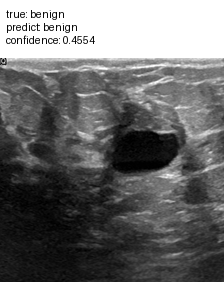
\includegraphics[width=0.42\textwidth]{report_images/classification_benign_correct.png}
\caption{Ví dụ output classification. Mô hình dự đoán đúng lớp \textit{benign}; confidence còn tương đối thấp, cho thấy mô hình vẫn chưa thật sự chắc chắn ở một số mẫu.}
\end{figure}

\begin{figure}[H]
\centering
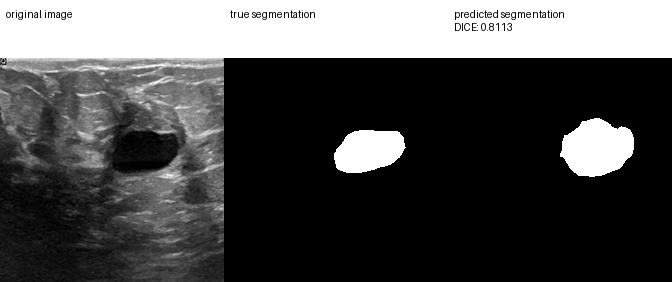
\includegraphics[width=0.98\textwidth]{report_images/segmentation_benign_good.png}
\caption{Ví dụ segmentation tương đối tốt trên mẫu benign. Mask dự đoán gần với mask thật và đạt Dice 0.8113.}
\end{figure}

\begin{figure}[H]
\centering
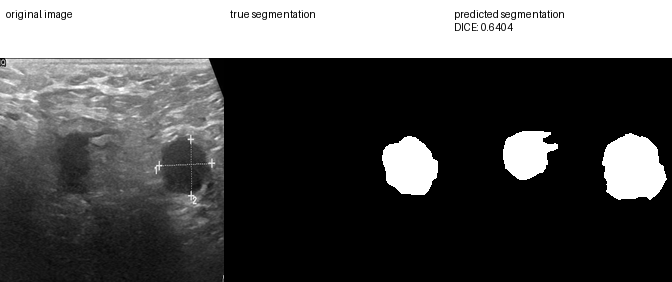
\includegraphics[width=0.98\textwidth]{report_images/segmentation_malignant_partial.png}
\caption{Ví dụ segmentation trên mẫu malignant. Mô hình xác định được vùng tổn thương chính nhưng dự đoán bị tách thành nhiều vùng, Dice 0.6404. Đây là một minh chứng cho việc segmentation đã học được tín hiệu bước đầu nhưng còn cần cải thiện về hình dạng và tính liền mạch của mask.}
\end{figure}

\begin{figure}[H]
\centering
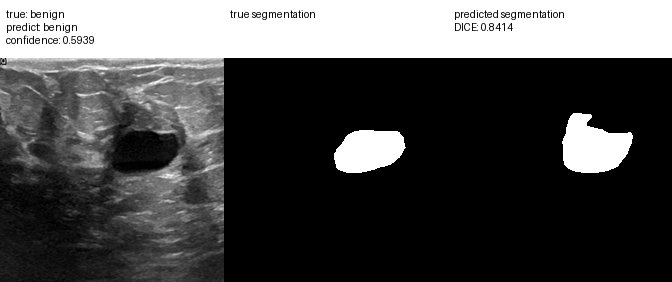
\includegraphics[width=0.98\textwidth]{report_images/multitask_benign_correct.png}
\caption{Ví dụ output multi-task. Cùng một ảnh đầu vào, mô hình vừa dự đoán đúng lớp \textit{benign}, vừa tạo mask segmentation với Dice 0.8414.}
\end{figure}

\begin{figure}[H]
\centering
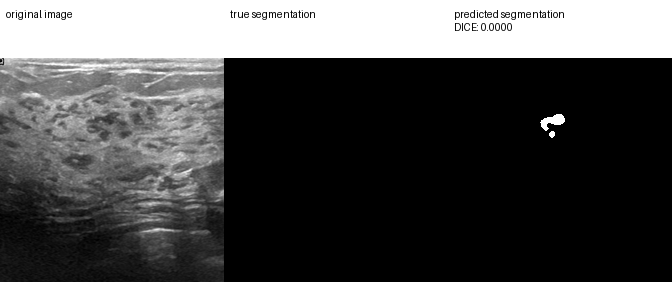
\includegraphics[width=0.98\textwidth]{report_images/segmentation_normal_false_positive.png}
\caption{Ví dụ hạn chế hiện tại trên mẫu normal. Mask thật không có vùng tổn thương nhưng mô hình vẫn sinh một vùng dự đoán nhỏ, Dice 0.0000. Trường hợp này cho thấy cần cải thiện khả năng xử lý ảnh normal và giảm false positive.}
\end{figure}

Nhìn chung, các hình trên cho thấy pipeline đã tạo được output trực quan đầy đủ. Tuy nhiên, kết quả segmentation chưa đồng đều giữa các mẫu: có trường hợp Dice cao, có trường hợp mask bị tách vùng hoặc sinh false positive. Vì vậy, ở giai đoạn tiếp theo nhóm cần tập trung vào loss segmentation, threshold, cân bằng dữ liệu/mask và phân tích trực quan có hệ thống hơn.

Các hình được sử dụng trực tiếp trong report đã được đóng gói riêng tại \path{report_images/}. Các thư mục output đầy đủ vẫn được giữ lại để kiểm tra thêm:

\begin{itemize}
    \item \path{report_images/}
    \item \path{lightweight-medical-model/outputs/busi/classification/img_224/test_images/}
    \item \path{lightweight-medical-model/outputs/busi/segmentation/img_224/test_images/}
    \item \path{lightweight-medical-model/outputs/busi/multi/img_224/test_images/}
\end{itemize}

\subsection{Artifact đã tạo}

\begin{table}[H]
\centering
\caption{Artifact chính đã có}
\renewcommand{\arraystretch}{1.25}
\begin{tabular}{p{4.2cm} p{9.8cm}}
\toprule
\textbf{Task} & \textbf{Artifact} \\
\midrule
Classification & \path{lightweight-medical-model/outputs/busi/classification/img_224/cbam/run_1/best_model.pt} \\
Segmentation & \path{lightweight-medical-model/outputs/busi/segmentation/img_224/cbam/best_model.pt} \\
Multi-task & \path{lightweight-medical-model/outputs/busi/multi/img_224/cbam/seg_weight_1/best_model.pt} \\
Logs và metrics & \path{lightweight-medical-model/outputs/busi/*/result.csv} và \path{epoch_log.csv} tương ứng. \\
\bottomrule
\end{tabular}
\end{table}

% =========================================================
\section{Cải tiến dự kiến}

\begin{expectbox}{Hướng cải tiến tiếp theo}
Các bước tiếp theo tập trung vào nâng chất lượng segmentation, tăng độ tin cậy của classification và bổ sung khả năng giải thích mô hình.
\end{expectbox}

\begin{enumerate}[label=\textbf{G\arabic*.}]
    \item \textbf{Cải thiện mô hình và quá trình huấn luyện}. Nhóm sẽ ưu tiên nâng chất lượng segmentation và tối ưu multi-task model. Cụ thể, phần segmentation sẽ được thử thêm Dice Loss hoặc Dice + BCE Loss, tinh chỉnh threshold, kiểm tra class/mask imbalance và xử lý tốt hơn các ảnh \textit{normal} có mask rỗng. Với multi-task learning, nhóm sẽ thử các giá trị \(\lambda\) khác nhau cho segmentation loss và xem xét checkpoint theo cả validation accuracy lẫn validation Dice, thay vì chỉ ưu tiên classification.

    \item \textbf{Củng cố đánh giá thực nghiệm}. Để kết quả có sức thuyết phục hơn, nhóm sẽ bổ sung confusion matrix, per-class precision/recall/F1, Macro-F1, sensitivity và specificity, trong đó ưu tiên kiểm tra riêng lớp \textit{malignant}. Ngoài ra, classification-only và multi-task sẽ được chạy lại với nhiều seed trên cùng split để báo cáo mean \(\pm\) std, tránh kết luận dựa trên một lần chạy. Nhóm cũng sẽ bổ sung baseline/ablation như Cross Entropy so với Focal Loss, tắt/bật CBAM, thay đổi \(\lambda\), và nếu đủ tài nguyên thì thêm ResNet-18, MobileNetV2 hoặc U-Net nhỏ.

    \item \textbf{Làm rõ tính lightweight của mô hình}. Bên cạnh số tham số và kích thước checkpoint đã báo cáo, nhóm sẽ bổ sung FLOPs/MACs, thời gian inference và so sánh với một số baseline chuẩn. Mục tiêu là biến nhận định ``lightweight'' từ mô tả định tính thành bằng chứng định lượng có thể đối chiếu.

    \item \textbf{Bổ sung XAI và phân tích trực quan}. Nhóm sẽ triển khai Grad-CAM cho nhánh classification để kiểm tra mô hình có tập trung vào vùng tổn thương hay không. Các kết quả trực quan sẽ được tổ chức theo nhóm mẫu đúng/sai, từng lớp bệnh, ảnh gốc, mask thật, mask dự đoán và Grad-CAM. Nếu Grad-CAM lệch khỏi mask tổn thương, nhóm sẽ phân tích khả năng mô hình đang học shortcut từ texture, nhiễu hoặc artifact trong ảnh siêu âm.

    \item \textbf{Áp dụng thêm data augmentation theo hướng proposal}. Sau khi baseline multi-task ổn định, nhóm sẽ quay lại khai thác ý tưởng augmentation từ proposal/paper ban đầu, nhưng chỉ chọn một số phương pháp phù hợp với tài nguyên hiện có thay vì so sánh toàn bộ augmentation policy. Các phép ưu tiên gồm rotation nhỏ, brightness/contrast nhẹ, shift/scale vừa phải và speckle noise. Với segmentation/multi-task, augmentation phải được áp dụng đồng bộ cho ảnh và mask để tránh làm lệch vùng tổn thương.
\end{enumerate}

% =========================================================
\section{Kết luận cập nhật}

Tính đến thời điểm hiện tại, nhóm đang ở giai đoạn \textbf{hoàn thành prototype end-to-end} của hướng triển khai mới. Nói cách khác, phần cốt lõi để chứng minh pipeline chạy được đã hoàn thành: dữ liệu BUSI đã được preprocess, mô hình lightweight đã được xây dựng, ba task classification/segmentation/multi-task đã được huấn luyện và các script test đã xuất được ảnh trực quan.

\begin{table}[H]
\centering
\caption{Vị trí hiện tại trong plan tổng thể}
\renewcommand{\arraystretch}{1.25}
\begin{tabular}{p{3.2cm} p{5.4cm} p{6.2cm}}
\toprule
\textbf{Mốc} & \textbf{Mục tiêu} & \textbf{Trạng thái hiện tại} \\
\midrule
Mốc 1 & Chuẩn bị dữ liệu và baseline chạy được. & Đã hoàn thành: dữ liệu BUSI có đủ train/val/test, classification baseline đã có kết quả. \\
Mốc 2 & Mở rộng sang segmentation để tận dụng mask. & Đã hoàn thành bước đầu: segmentation chạy được nhưng chất lượng mask chưa ổn định. \\
Mốc 3 & Kết hợp classification và segmentation bằng multi-task learning. & Đã hoàn thành prototype: multi-task có kết quả classification cao hơn baseline trong lần chạy hiện tại, segmentation ở mức cần cải thiện. \\
Mốc 4 & Phân tích sâu, cải thiện model và bổ sung XAI. & Đang chuẩn bị triển khai: Grad-CAM, cải thiện segmentation loss, thêm metric y khoa. \\
Mốc 5 & Hoàn thiện báo cáo cuối và đánh giá hệ thống. & Chưa hoàn thành: cần thêm thí nghiệm, phân tích lỗi và trực quan hóa giải thích. \\
\bottomrule
\end{tabular}
\end{table}

So với proposal ban đầu, phạm vi đã được điều chỉnh do giới hạn tài nguyên huấn luyện: thay vì tập trung vào ResNet/EfficientNet và nhiều augmentation policy, nhóm chuyển sang lightweight multi-task model để tận dụng cả nhãn classification và mask segmentation. Paper \texttt{mednet.pdf} đóng vai trò cầu nối cho thay đổi này, vì cung cấp cơ sở để ưu tiên một mô hình định hướng cho ảnh y khoa thay vì chỉ dựa trên backbone tổng quát. Đây không phải là thay đổi rời khỏi bài toán ảnh siêu âm y khoa, mà là điều chỉnh để phù hợp hơn với tài nguyên thực tế và khai thác đầy đủ hơn dữ liệu BUSI.

Kết quả multi-task hiện tại là tín hiệu ban đầu đáng chú ý khi đạt Test Acc 81.67\% và Test AUC 0.9129 trong một lần chạy. Tuy nhiên, nhóm chưa xem đây là bằng chứng cuối cùng rằng multi-task vượt trội hơn classification-only, vì chưa có nhiều seed, confusion matrix, per-class metric và kiểm định tính ổn định. Phần segmentation vẫn là điểm yếu chính: một số mẫu cho Dice tốt, nhưng một số mẫu normal hoặc biên tổn thương không rõ vẫn tạo false positive hoặc mask chưa đúng hình dạng. Vì vậy, giai đoạn tiếp theo sẽ không chỉ là chạy thêm model, mà là \textbf{phân tích lỗi có hệ thống}: xem mô hình sai ở nhóm ảnh nào, mask sai theo kiểu nào, lớp \textit{malignant} có bị bỏ sót hay không, và Grad-CAM có tập trung vào vùng tổn thương hay không.

Tóm lại, nhóm hiện đã đi qua giai đoạn ``xây pipeline và chứng minh chạy được'', đang bước vào giai đoạn ``củng cố bằng chứng thực nghiệm''. Trọng tâm gần nhất là biến kết quả prototype thành kết quả nghiên cứu có thể bảo vệ trước phản biện: so sánh công bằng hơn, thêm per-class metric, đánh giá nhiều seed, cụ thể hóa tính lightweight bằng FLOPs/inference time, cải thiện segmentation và bổ sung Grad-CAM/XAI.

\end{document}
